\section{Casi d'uso}

Il gruppo di analisi ha identificato diversi casi d'uso nel capitolato d'appalto proposto, raggruppandoli in tipologie distinte.
Di seguito vengono riportate le nomenclature utilizzate per indicare i casi d'uso, la loro struttura, e gli attori che interagiscono con il Sistema.

\subsection{Nomenclatura dei casi d'uso}
\begin{itemize}
	\item \textbf{UCG} : indica un caso d'uso$^G$ strettamente legato all'Utente generico$^G$.
	\item \textbf{UCA} : indica un caso d'uso strettamente legato all'Utente autenticato$^G$.
	\item \textbf{UCB} : indica un caso d'uso strettamente legato all'Utente base$^G$.
	\item \textbf{UCR} : indica un caso d'uso strettamente legato all'Utente ristoratore$^G$.
	\item \textbf{UCE} : indica un caso d'uso strettamente legato ad un errore.
\end{itemize}
\subsection{Struttura dei casi d'uso}
I casi d'uso sono strutturati nel seguente modo:
\begin{itemize}
	\item \textbf{Titolo:} fornito di un codice identificativo e di un nome esplicativo per agevolare il tracciamento.
	\item \textbf{Attori:} diverse tipologie di utenti che interagiscono con il sistema, suddivisi in:
	      \begin{itemize}
		      \item Attore$^G$ primario: colui che interagisce attivamente con il Sistema dall'esterno.
		      \item Attore secondario: possono anche non essere presenti.
		            Sono sempre esterni, ma non interagiscono attivamente con il Sistema; invece, interagiscono per il raggiungimento dello scopo dell'attore primario o per aiutarlo.
	      \end{itemize}
	\item \textbf{Precondizioni:} stato in cui si deve trovare il Sistema affinchè una funzionalità sia disponibile ad un attore.
	\item \textbf{Postcondizioni:} serie di informazioni che rappresentano lo stato del Sistema dopo l'esecuzione del caso d'uso.
	\item \textbf{Scenario principale:} sequenza di azioni dettagliata che descrive il \textit{workflow} della funzionalità.
	\item \textbf{Descrizione:} note aggiuntive inserite quando si ritiene utile ampliare la spiegazione per approfondire la comprensione del caso d'uso.
	\item \textbf{Scenario secondario:} scenario che inizialmente ha lo stesso \textit{workflow} di quello principale ma che, ad un tratto, diverge , solitamente relativo a errori.
	\item \textbf{\textit{Trigger}:} evento scatenante che provoca l'esecuzione automatica del caso d'uso.
	\item \textbf{Inclusione:} è una relazione in cui un caso d'uso (il caso d'uso di base) include la funzionalità di un altro caso d'uso (il caso d'uso di inclusione).
	      La relazione di inclusione supporta il riutilizzo della funzionalità in un modello di caso d'uso.
	\item \textbf{Estensione:} è una relazione per specificare che un caso d'uso (estensione) estende il comportamento di un altro caso d'uso (base).
	      La relazione di estensione specifica che l'incorporazione del caso d'uso dell'estensione dipende da ciò che accade quando viene eseguito il caso d'uso di base.
	\item \textbf{Generalizzazione:} è una relazione in cui un elemento del modello (il figlio) è basato su un altro elemento del modello (il genitore).
	      Le relazioni di generalizzazione vengono usate per indicare che il figlio riceve tutti gli attributi, le operazioni e le relazioni definiti nel genitore.
\end{itemize}

\newpage
\subsection{Attori}

\begin{figure}[h]
	\centering
	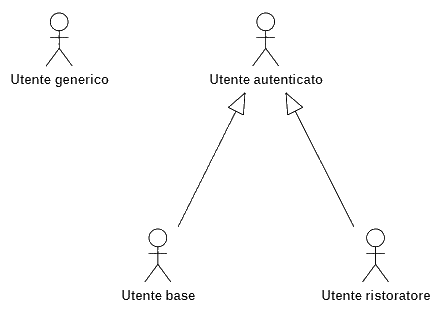
\includegraphics[width=0.6\textwidth]{./uml/gerarchia_attori.png}
	\caption{Gerarchia degli attori}
\end{figure}

Gli attori identificati per il sistema e le relative dipendenze sono i seguenti:
\begin{itemize}
	\item \textbf{Utente generico}: è un utente che non ha effettuato l'accesso al
	      Sistema. Può essere un utente non registrato o un utente registrato che non ha
	      ancora effettuato l'accesso;

	\item \textbf{Utente autenticato}: l'Utente autenticato rappresenta un Utente
	      base oppure un Utente ristoratore che ha effettuato l'accesso al Sistema.

	\item \textbf{Utente base}: l'Utente base è colui che può effettuare l'accesso al Sistema e può
	      effettuare delle prenotazioni e attività correlate. L'Utente base rappresenta
	      il cliente$^G$ del ristorante;

	\item \textbf{Utente ristoratore}: l'Utente ristoratore è colui che può gestire il proprio ristorante e le
	      prenotazioni ad esso associate. L'Utente ristoratore rappresenta il gestore del
	      ristorante;
\end{itemize}

\newpage
\subsection{Casi d'uso}
